\documentclass[noshadow]{LSRslides}
% use class option 'longpres' if you want to use subsections
% use class option 'noshadow' if you want to use blocks without shadow
% beameroptions can be used, e.g. 'handout'
\graphicspath{{logos/}{pictures/}}
\addbibresource{ref.bib}
\title{Technology of Autonomous Systems}

\presenter{O. Ayan, J. Heuser, R.Lauer, M. Sezer}{}
%\addauthor[1]{D. Carton}{}


\addaffiliations[]{Chair of Automatic Control Engineering}{Technische Universität München}


\occasion{Final presentation}

%% \date{month}{day}{year}
\date{20}{01}{2015}

% both packs for subfigure 
%(the subfigure and subfig packages are deprecated and shouldn't be used any more)
\usepackage{caption}
\usepackage{subcaption}
\usepackage{psfrag}
\usepackage{booktabs}
\usepackage{tabulary}
\usepackage[inline]{asymptote}
\usepackage{fancybox}
\usepackage{biblatex}
\usepackage{tikz}
\usetikzlibrary{calc,shapes,arrows,positioning,shapes.geometric}

% include video
\usepackage{multimedia} %% only OKULAR READER can show video!!


% %to display vectors as bold 
\renewcommand{\vec}[1]{\boldsymbol{#1}} 
\renewcommand{\d}{\, \mathrm{d}} % for integrals 
%\newcommand{\sgn}{\operatorname{sgn}}
\DeclareMathOperator{\sgn}{sgn}
\newcommand{\co}{\operatorname{c}}
\newcommand{\si}{\operatorname{s}}


%%%%%%%%%%%%%%%%%%%%%%%%%%%%%%%%%%%%%%%%%%%%%%%%%%%%%%%%%%%%%%%%%%%%%%%%%%%%%%%%
\begin{document}


\begin{frame}
    \titlepage
\end{frame}

\begin{frame}
	\frametitle{Talk Overview}
\tableofcontents
\end{frame}

\section{Parallel Parking Approach}
\begin{frame}
\frametitle{Parallel Parking Approach I}
\begin{figure}
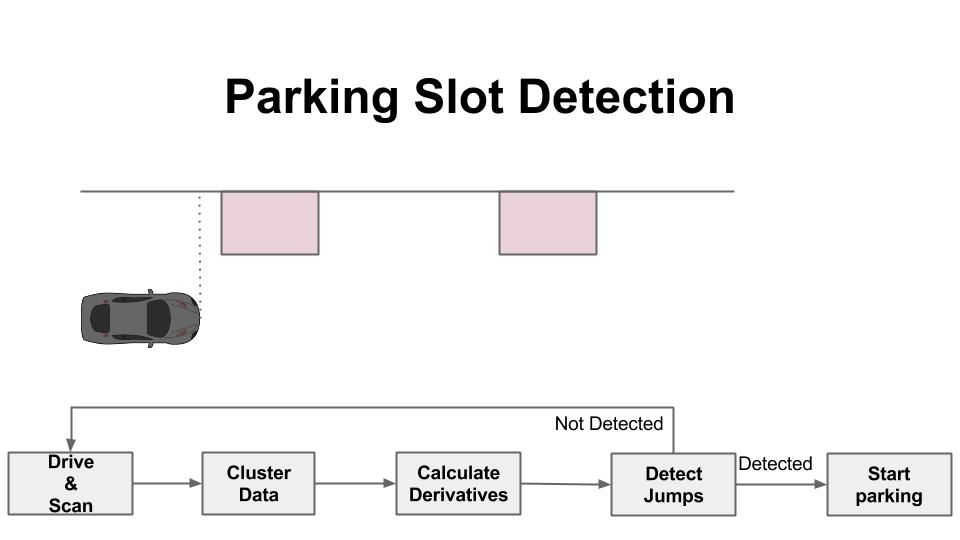
\includegraphics[width = 1\textwidth]{Parking_Detection_TAS.jpg}
\end{figure}
\end{frame}

\begin{frame}
\frametitle{Parallel Parking Approach II}
%\begin{columns}
%\column{0.5\textwidth}
\begin{figure}
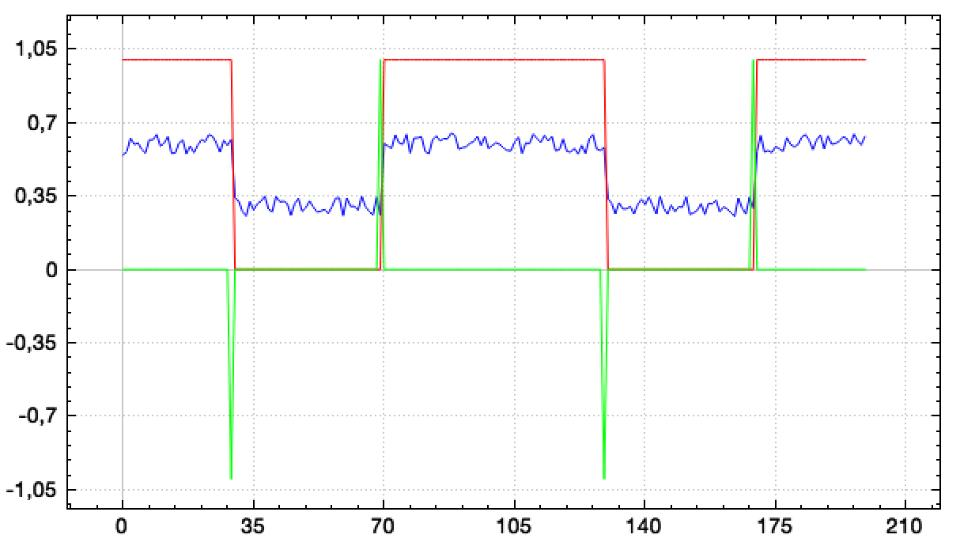
\includegraphics[width = 0.5\textwidth]{Parking_Detection_TAS_21.jpg}
\end{figure}

%\column{0.5\textwidth}
\begin{figure}
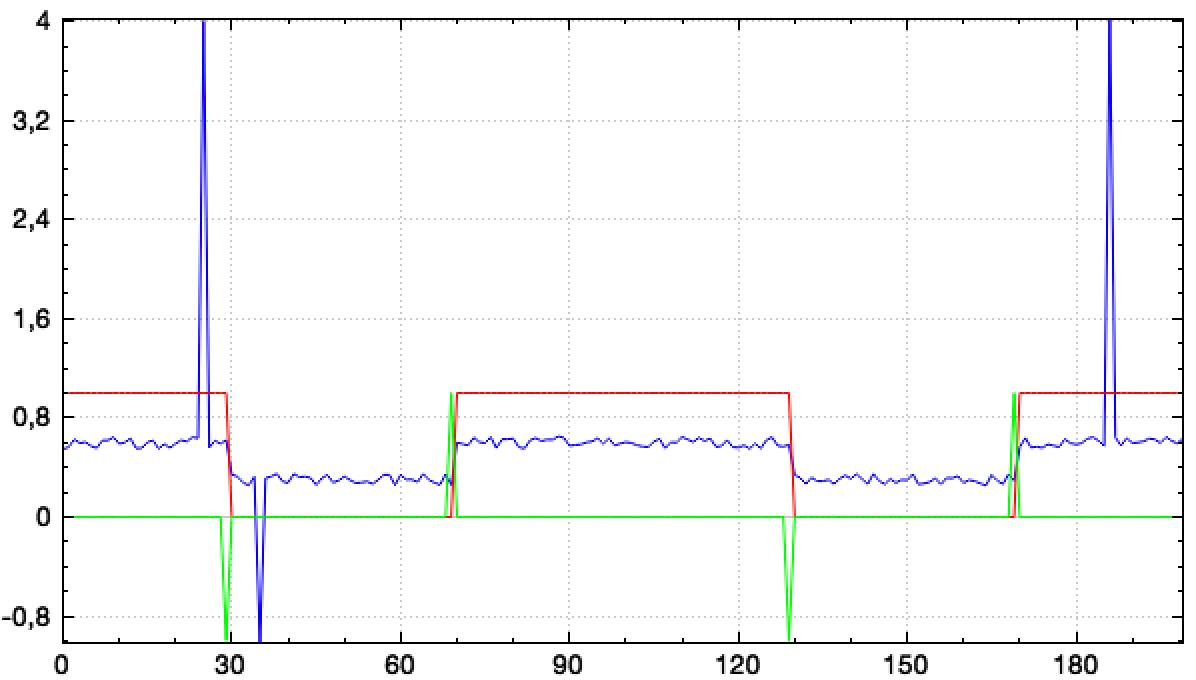
\includegraphics[width = 0.5\textwidth]{Parking_Detection_TAS_22.jpg}
\end{figure}

%\end{columns}
\end{frame}

\begin{frame}
\frametitle{Parallel Parking Approach III}
\begin{columns}
\column{0.5\textwidth}
\footnotesize
\begin{enumerate}
\item Parking lot was detected
\item Car positions and ranges at 1st and 2nd jump were stored
\item Calculate corners of parking lot from that data
\item Final position (4) is center of parking lot
\item Third (3) way point is at the back of parking lot (safety distances: side $\approx 6cm$, back $\approx 4cm$)
\item x coordinate of starting point (1) equals distance to wall $\rightarrow$ calculate y coordinate using the turning circle of the car
\item Wheel turning point (2) is point of intersection of circles
\end{enumerate}

\column{0.55\textwidth}
\begin{figure}
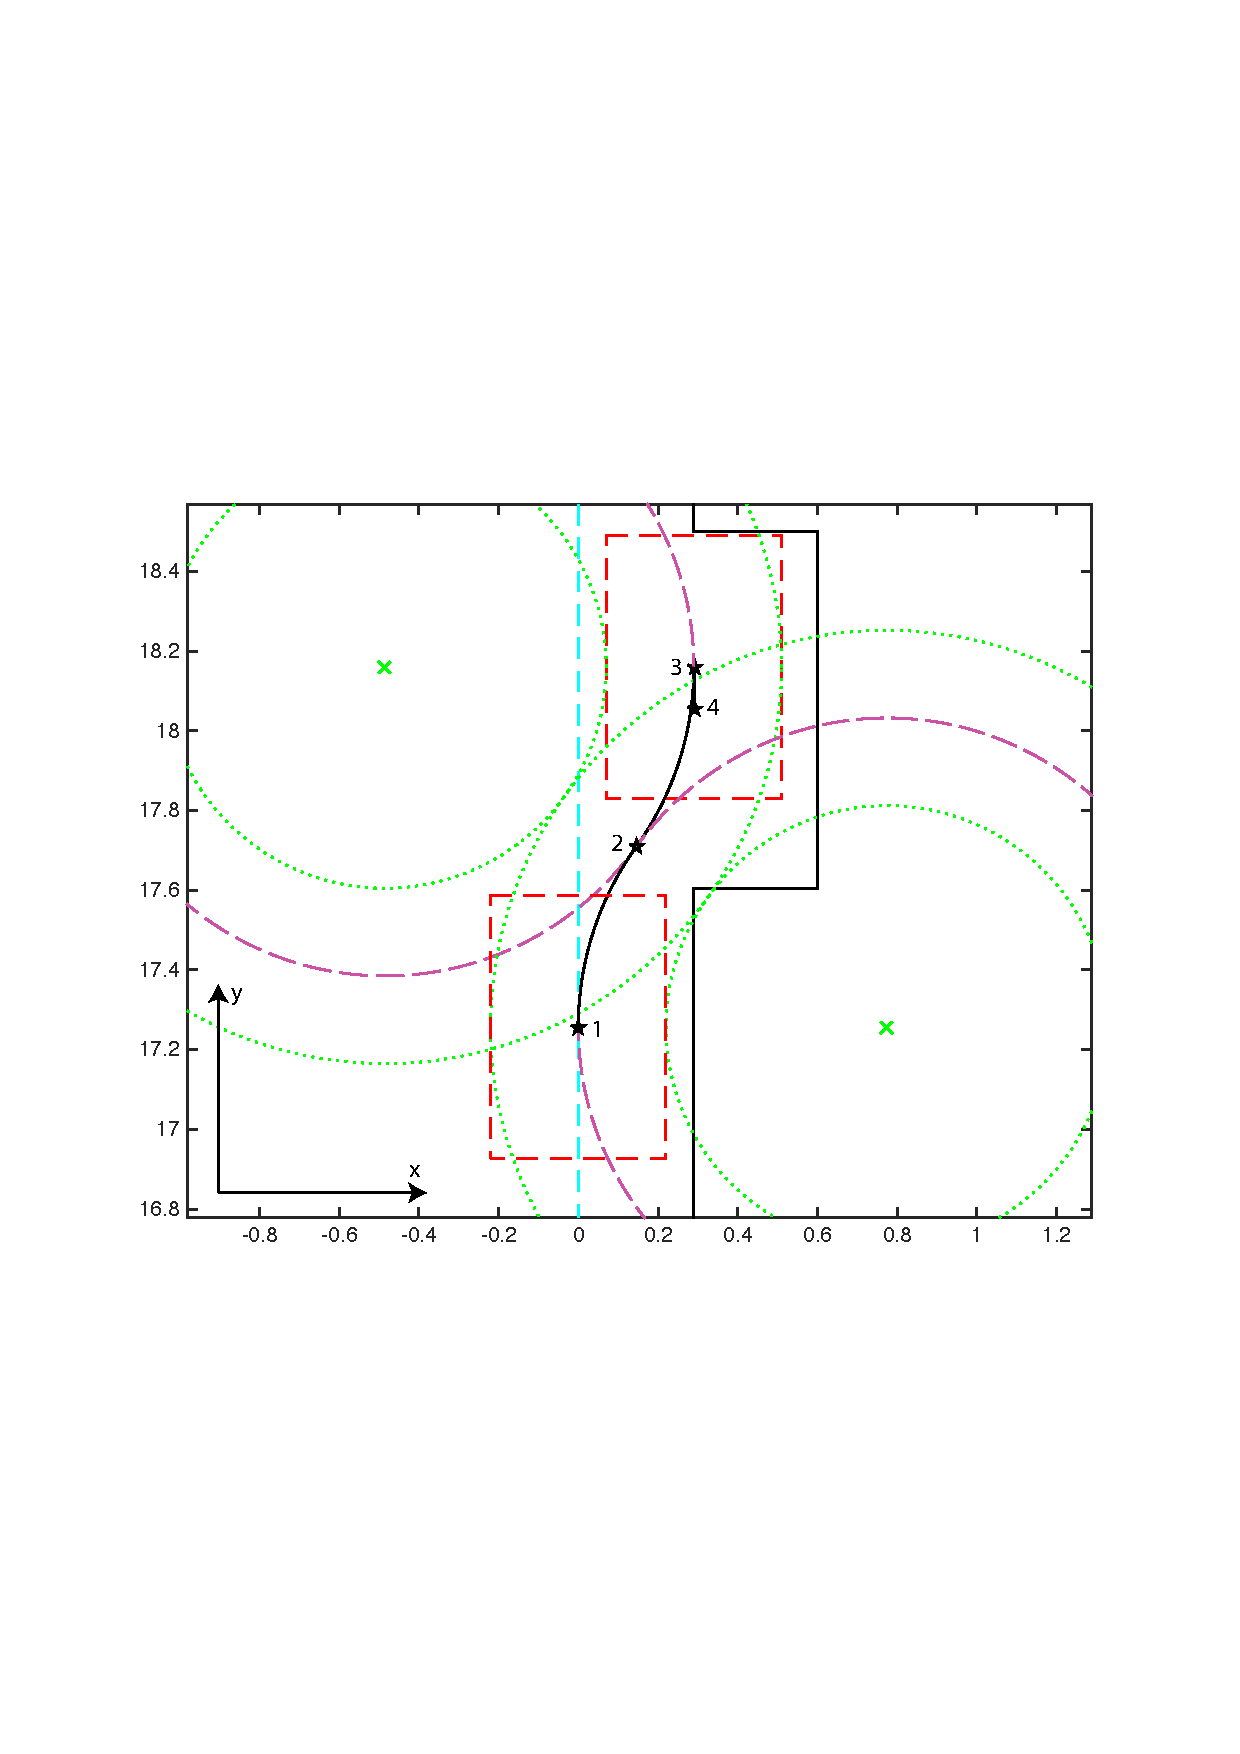
\includegraphics[width = 1\textwidth]{parking_plot.pdf}
\end{figure}

\end{columns}
\end{frame}


\section{Indoor Wi-Fi Positioning}
\begin{frame}
\frametitle{Indoor Wi-Fi Positioning}

	\textbf{Trilateration}

   
   \begin{itemize}
	\item Based on radio propagation model: 
	$\text{Intensity} \propto \frac{1}{\text{Distance}^2}$
	\item Requires line of sight, unusable due to deviation of signal strength
\end{itemize}
\textbf{Pattern Matching}
\begin{columns}
	\column{0.5\textwidth}
\vspace*{-4mm}	
	\begin{figure}
      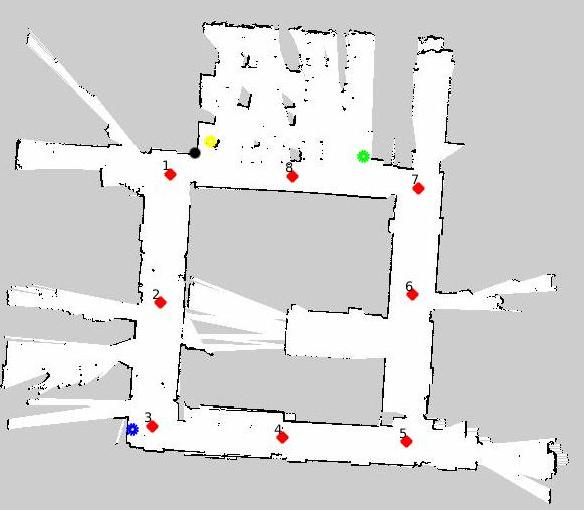
\includegraphics[scale=0.24,left]{DatabaseAndRouterPosNoTitleNEW.jpg} 
   \end{figure}
	
	
	\column{0.5\textwidth}
	
	%\centering
	\vspace*{-4mm}
	\begin{figure}
      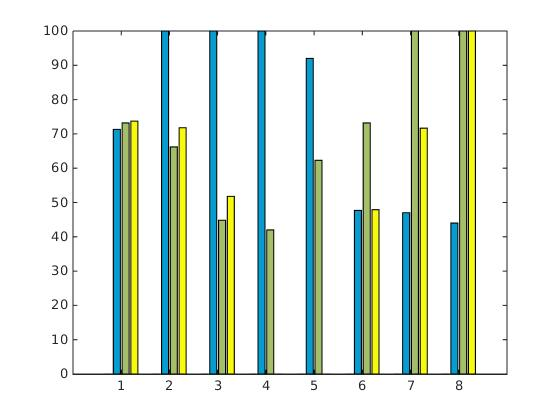
\includegraphics[scale=0.25,left]{DatabaseBarDiagramNoTitle.jpg} 
   \end{figure}
   \end{columns}
   
   \begin{itemize}
	\item Build a database and use nearest neigbour pattern matching (Fingerprinting model)
\end{itemize}
		
\end{frame}

\begin{frame}
\frametitle{Indoor Wi-Fi Positioning}
\textbf{In practice: }
 \begin{itemize}
	\item Able to locate the car in its initial position (x,y) for given task, in general accuracy limited by database
	\item Tracking of the cars movement fails due to too few accesspoints used (less features to compare) and rather slow update of wifi-signals  
	\item performance could be improved by using more accesspoints to generate more robust features, k-nearest neigbour position estimate ($k>1$) (or even weighted-KNN \cite{shin12}) and a bigger database
\end{itemize}

\end{frame}

\section{Adaptive Velocity Controller}
\begin{frame}
\frametitle{Adaptive Velocity Controller  - Overview}


\begin{columns}
	\column{0.7\textwidth}	
	
\begin{itemize}
\small
	\item Dynamically reconfigurable node that controls the servo velocity based on
	\begin{itemize}
	\item Global plan curvature
	\item Local plan curvature
	\item Nearest obstacle distance in virtual lane
	\end{itemize}
	\item Linear mapping of cmd\_vel
	\item Parameters subject to optimize

\end{itemize}

\begin{figure}
	%\raggedright
      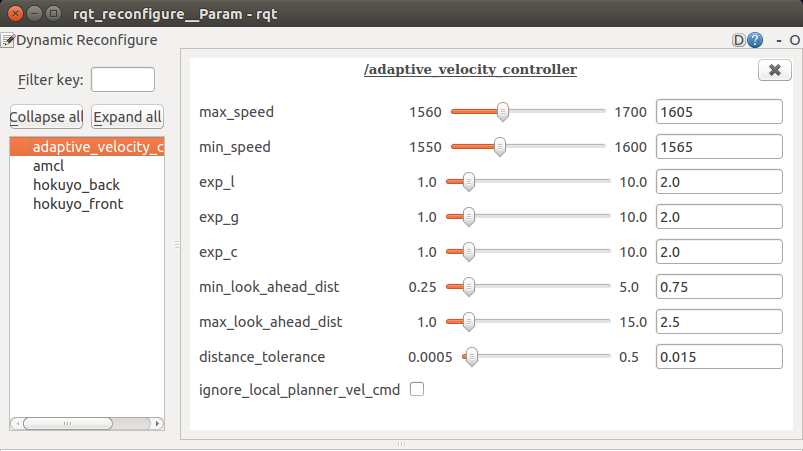
\includegraphics[scale=0.3]{adaptive_velocity_rqt.png} 
     % \caption{This is a picture!}
   \end{figure}

	\column{0.5\textwidth}
	%\vspace*{-15mm}
	%\hspace*{13mm}
	\centering
	% figure of coord systems of ellipse
	\begin{figure}
	%\raggedright
      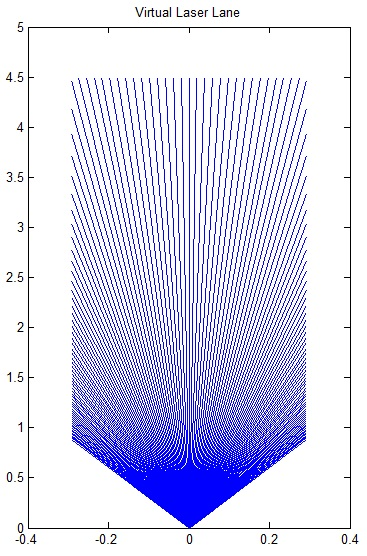
\includegraphics[scale=0.45]{virtual_lane.jpg} 
     % \caption{This is a picture!}
   \end{figure}	
\end{columns}

%\vspace*{-7mm}

\end{frame}

\begin{frame}
\frametitle{Adaptive Velocity Controller - Program Flow}

\tikzstyle{block} = [rectangle, draw, text width = 1.5 cm, text centered, rounded corners, minimum height=3.5em]
\tikzstyle{line} = [draw, -latex']
\tikzstyle{cloud} = [draw, ellipse, node distance=1.5cm,
    minimum height=2em]
\tikzstyle{baklava} = [diamond, minimum width=0.5cm, minimum height=0.5cm, text centered, draw=black]

\vspace{-0.7cm}
\begin{figure}
\scriptsize
\begin{tikzpicture}[node distance = 2.5 cm, auto]
\node [block, color = blue] (dynamic) {Dynamic Reconfigure};
\node [block, color = blue, right of=dynamic, xshift=-0.5cm] (params) {Get Parameters};
\node [block, color = blue, right of=params, xshift=-0.5cm] (lookup) {Compute Lookup Table};
\node [block, below of=params, yshift=0.76cm] (scan) {Scan Callback};
\node [cloud, right of=scan, xshift=2.15 cm, text width = 2.5cm, text centered] (clearpath) {Clear Path Ratio};
\node [block, below of=scan, yshift=1.25cm] (global) {Global Plan Callback};
\node [cloud, right of=global, xshift=2.15cm, text width = 2.5cm, text centered] (globalcurv) {Global Plan Curvature};
\node [block, below of=global, yshift=1.25cm] (local) {Local Plan Callback};
\node [cloud, right of=local, xshift=2.15cm, text width = 2.5cm, text centered] (localcurv) {Local Plan Curvature};
\node [block, right of=globalcurv, xshift=1cm] (compute) {Compute Servo Velocity};
\node [baklava, text width = 1.2cm, above of=compute] (cmdvel) {cmd\_vel from move\_base};

\path [line, color=blue] (dynamic) -- (params);
\path [line, dashed, color=blue] (params) -- (lookup);
\path [line] (clearpath.east) -- ($(compute.west) + (0,0.25)$);
\path [line] (globalcurv.east) -- (compute.west);
\path [line] (localcurv.east) -- ($(compute.west) + (0,-0.25)$);
\path [line] (scan) -- (clearpath);
\path [line] (global) -- (globalcurv);
\path [line] (local) -- (localcurv);
\path [line, dashed, color = blue] (lookup) |- ($(lookup.north) + (0,0.35)$) -- ($(params.north) + (0,0.35)$) -| (params.north);
\path [line] (lookup.south) |- ($(lookup.south) - (0,0.34)$) -- ($(scan.north) + (0,0.33)$) -| (scan.north);
\path [line, dashed] (cmdvel) -- (compute);
%\path [line] (dynamic) |- ($(lookup.south) + (0,-0.07)$);
\end{tikzpicture}
\end{figure}

\tiny
\textbf{SERVO VELOCITY:} \newline
$MIN\_SPEED + (SPEED-MIN\_SPEED)*(curv_l)^{exp\_l}*(curv_g)^{exp\_g}*(\frac{min\_obs\_dist}{MAX\_LAD})^{exp\_c}$

\end{frame}



% TO DO: Bibliography
%
\appendix
%\nocite{buss11}
%\nocite{bauer09}
\begin{frame}
	\frametitle{References}
	\printbibliography
\end{frame}


\end{document}
